\chapter{Regulacja procesu}
	\label{ch:reg}
	
	\section{Implementacja NPL}
		\label{sec:NPL}
		NPL jest algorytmem regulacji predykcyjnym z nieliniową predykcją i z linearyzacją oznacza to że do wyznaczania trajektori swobodnej (która zależy tylko od przeszłych sterowań) używamy nieliniowego modelu neuronowego:
		\begin{equation}
		\begin{tabular}{l}
		$y^0(k+p|k)=w20+w2*tanh(w10+w1*x(k+p))+dk$
		\end{tabular}
		\label{eq:NPL_y0}
		\end{equation}
		gdzie
		\begin{equation}
		\begin{tabular}{l}
		$dk = y(k)-y^M(k)$
		\end{tabular}
		\label{eq:dk}
		\end{equation}
		\begin{equation}
		\begin{tabular}{l}
		$x(k)=$ $\begin{bmatrix}u(min(k-\tau+p,k-1))\\u(min(k-\tau-1+p,k-1))\\y(k-1+p)\\y(k-2+p)\end{bmatrix}$
		\end{tabular}
		\label{eq:wesn}
		\end{equation}
		$p=$ ilość chwil w przyszłóść.
		Warto dodać, że we wzore \ref{eq:wesn} dla chwil czasu dalszych od $k$ zakłada się że $y(k+p)=y^0(k+p|k)$.\\
		Aby móc rozwiązać algorytm analitycznie dokonuje się linearyzacji wyjścia modelu. Współczynniki $b_3$,$b_4$,$a_1$,$a_2$ we wzorze
		\begin{equation}
		\begin{tabular}{l}
		$y(k)=b_3u(k-\tau)+b_4(k-\tau-1)-a_1y(k-1)-a_2y(k-2)$
		\end{tabular}
		\label{eq:NPL_wyjscielinear}
		\end{equation}
		otrzymuje się poprzez obliczenie pochodnej cząstkowej po odpowiednim wejściu modelu neuronowego. Mając obliczone współczynniki można użyć ich do wyznaczenia odpowiedzi skokowej ze wzoru
		\begin{equation}
		\begin{tabular}{l}
		$s_j(k)=\sum\limits_{i=1}^{min(j,n_B)}b_i(k)-\sum\limits_{i=1}^{min(j-1,n_A)}s_{j-i}(k)$
		\end{tabular}
		\label{eq:NPL_odpowiedzskok}
		\end{equation}
		których można użyć do wypełnienia macierzy dynamicznej M.
		
		\begin{equation}
		\boldsymbol{M}=\left[
		\begin{array}
		{cccc}
		s_{1} & 0 & \ldots & 0\\
		s_{2} & s_{1} & \ldots & 0\\
		\vdots & \vdots & \ddots & \vdots\\
		s_{N} & s_{N-1} & \ldots &  s_{N-N_{\mathrm{u}}+1}
		\end{array}
		\right]_{\mathrm{NxN_u}}
		\label{Mm}
		\end{equation}
		
		Na koniec można obliczyć optymalne przyszłe sterowania(przy zadanych horyzontach predykcji N i sterowania Nu oraz współczynniku kary $\lambda$). 
		\begin{equation}
		\begin{tabular}{l}
		$dU=K*(Y_{zad}(k)-Y^0)$
		\end{tabular}
		\label{eq:NPL_du}
		\end{equation}
		gdzie $Y_{zad}(k)$ to wektor długości N zawierający aktualną wartość zadaną, $Y^0$ to wektor N przyszłych, predykowanych wartości wyjścia oraz
		\begin{equation}
		\begin{tabular}{l}
		$K=(M'*M+\lambda I)^{-1}*M'$
		\end{tabular}
		\label{eq:NPL_K}
		\end{equation}
	
		
		
	\section{Strojenie NPL}
		\label{sec:stroj_NPL}
		Regulator NPL został nastrojony z użyciem sieci neuronowej wytrenowanej algorytmem BFGS z użyciem rekurencji opisanej w sekcji \ref{sec:bfgs}. Strojenie regulatora NPL rozpoczęliśmy od parametrów $N=15$, $N_u=2$ oraz $\lambda=1$. Przebieg dla tych wartości zaprezentowany jest poniżej (rys. \ref{fig:NPL0}). Jak widać już od samego początku przebieg regulacji nie jest zły, aczkolwiek sterowanie jest zdecydowania zbyt ostre. Błąd o wartości 74.554 na 600 próbkach nie jest idealny, ale akceptowalny.
		
		\begin{figure}[h!]
			\centering
			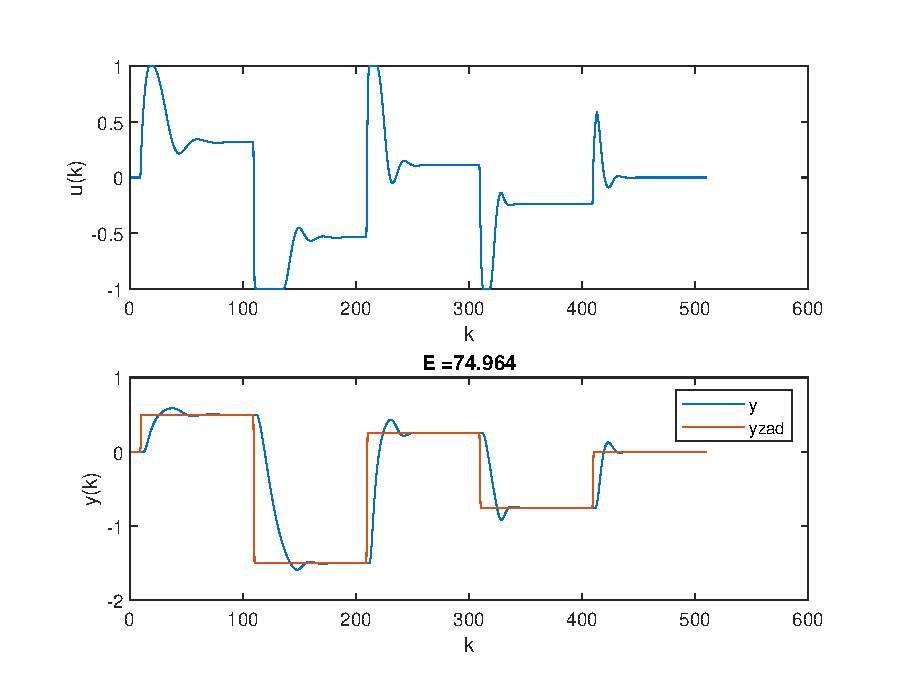
\includegraphics[width=0.7\linewidth]{img/strojenieNPL_N_15_Nu_2_lam_1.eps}
			\caption{Działanie regulatora NPL z nastawami N=15, Nu=2, $\lambda$=1}
			\label{fig:NPL0}
		\end{figure}
		
		W celu zmniejszenia gwałtowności sterowania postanowiliśmy zwiększać wartość $\lambda$ do czasu od sterowanie złagodnieje. Należy oczywiśćie pamiętać, że im większy jest parametr $\lambda$, tym regulator będzie wolniejszy. Kompromis pomiędzy szybkością (błędem), a kształtem sygnału sterującego osiągneliśmy dla $\lambda=4$, błąd wynosił 75.8664. Przebieg zaprezentowany jest na rys. \ref{fig:NPL1}
		
		\begin{figure}[h!]
			\centering
			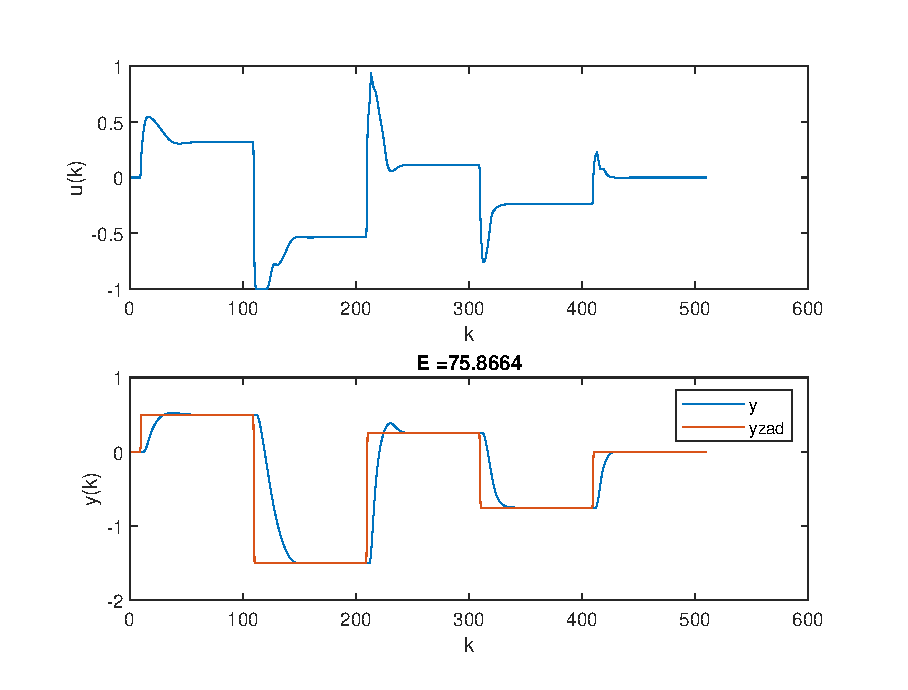
\includegraphics[width=0.7\linewidth]{img/strojenieNPL_N_15_Nu_2_lam_4.eps}
			\caption{Działanie regulatora NPL z nastawami N=15, Nu=2, $\lambda$=}
			\label{fig:NPL1}
		\end{figure}
		
		\newpage
		Teraz gdy sygnał sterowania jest już łagdoniejszy postanowiliśmy zbadać wpływ horyznto predykcji na jakość regulacji. Zauważyliśmy, że zarówno przy zmniejszaniu, jak i przy zwiększaniu wartości $N$, błąd rośnie, lecz dla dalszych horyzntów maleje przeregulowanie. Raz jeszcze postanowiliśmy znaleźć kompromis pomiędzy błędem, a przeregulowaniem. Sytuacją taką udało się osiągnąć dla $N=19$. Błąd wynosił 76.4364, natomiast przeregulowania było prawie niewidoczne.
		Przebieg ten można zobaczyć na rys. \ref{fig:NPL2}
		
		\begin{figure}[h!]
			\centering
			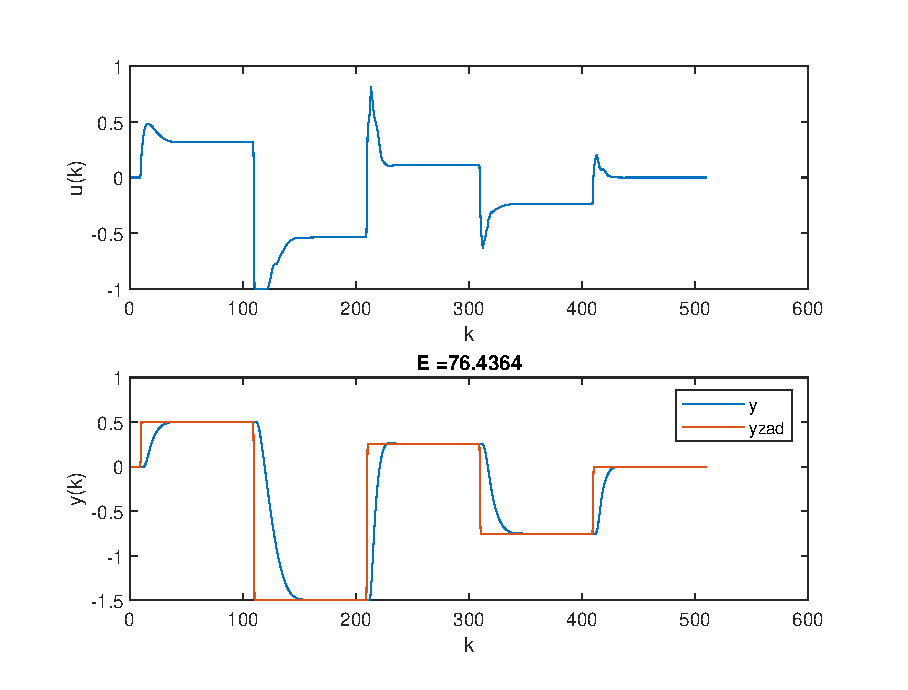
\includegraphics[width=0.7\linewidth]{img/strojenieNPL_N_19_Nu_2_lam_4.eps}
			\caption{Działanie regulatora NPL z nastawami N=19, Nu=2, $\lambda$=4}
			\label{fig:NPL2}
		\end{figure}
	
		\newpage
		Następnie postanowiliśmy dobrać horyzont sterowania. Niestety zarówno przy zwiększaniu jak i zmniejszaniu horyzontu jakość regulacji pogarszała się, co można zaobserwować na wykresach \ref{fig:NPL3} i \ref{fig:NPL4}. Dla Nu równego 1 błąd regulacji co prawda spadł, ale następują niekontrolowane, ostre skoki sterowania oraz znów pojawiły się przeregulowania. Dla Nu równego 3 wejscie prezentuje się podobnie, nastomiast ucierpiało wyjście.
		
		\begin{figure}[h!]
			\centering
			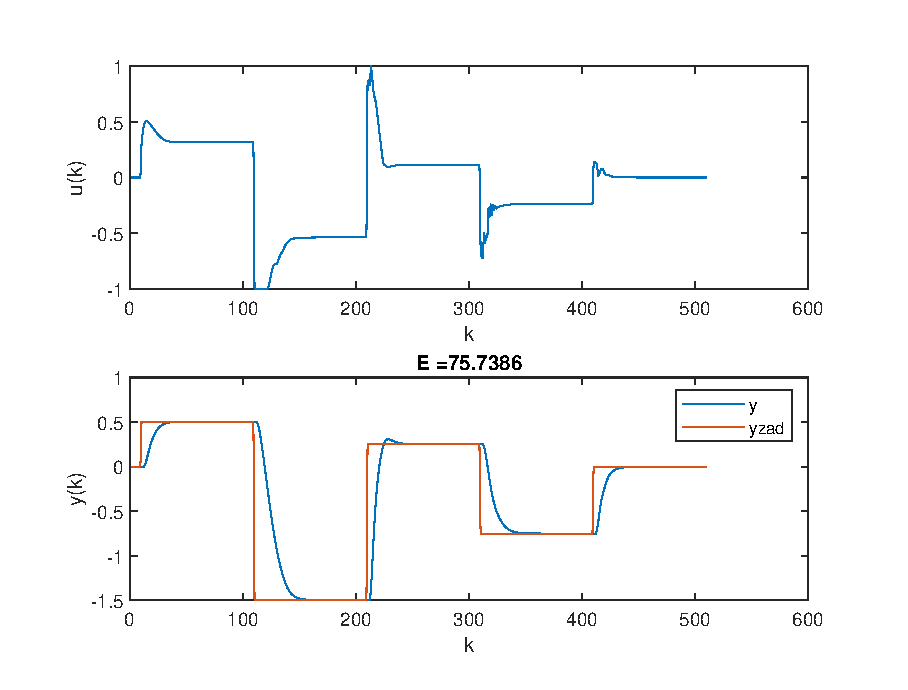
\includegraphics[width=0.7\linewidth]{img/strojenieNPL_N_19_Nu_1_lam_4.eps}
			\caption{Działanie regulatora NPL z nastawami N=19, Nu=1, $\lambda$=4}
			\label{fig:NPL3}
		\end{figure}
		
		\begin{figure}[h!]
			\centering
			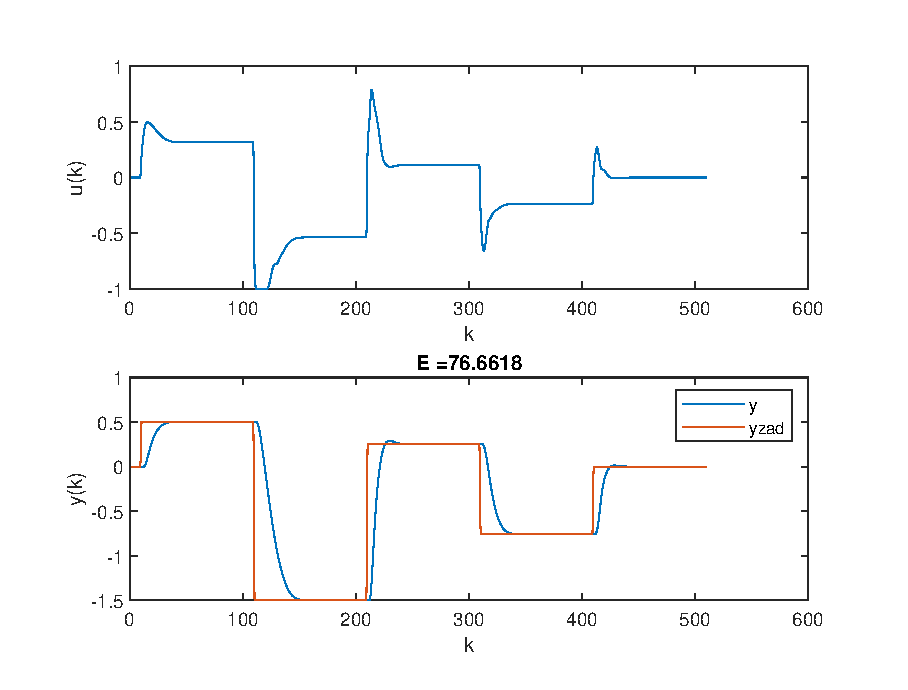
\includegraphics[width=\linewidth]{img/strojenieNPL_N_19_Nu_3_lam_4.eps}
			\caption{Działanie regulatora NPL z nastawami N=19, Nu=3, $\lambda$=4}
			\label{fig:NPL4}
		\end{figure}
		
	\newpage	
	\section{GPC}
		\label{sec:GPC}
		Algorytm regulacji GPC, różni się tym od NPL, że na całym horyzocnie predykcji korzysta się z liniowego modelu wyznaczonego metodą najmniejszych kwadratów. Jak można było zauważyć z rys. \ref{fig:mnk} taki model nie gwarantuje najlepszego odwzorowania obiektu, przez co jak można się domyślać jakość regulacji również może być gorsza.
		Do wyznaczania sterowania w wersji analitycznej wyznacza predykcje wyjscia modelu $N$ chwil do przodu ze wzoru
		\begin{equation}
		\begin{tabular}{l}
		$y^0(k+p|k)=b_3u(min(k-3+p,k-1))+b_4u(min(k-4+p),k-1)-a_1y(k-1+p)-a_2y(k-2+p)$
		\end{tabular}
		\label{eq:GPC_y0}
		\end{equation}
		oraz analogicznie do wzoru \ref{eq:NPL_y0} $y(k+p)=y^0(k+p|k)$. Parametry $a_i$ oraz $b_i$ otrzymywane są z metody najmniejszych kwadratów. Macierz dynamiczna jest stała i wyznaczana przy użyciu odpowiedzi skokowej ze wzoru \ref{eq:NPL_odpowiedzskok}. Na wykresie poniżej można zauważyć, że jakość regulacji w istocie pozostawia wiele do życzenia (rys \ref{fig:GPC}).
		
		\begin{figure}[h!]
			\centering
			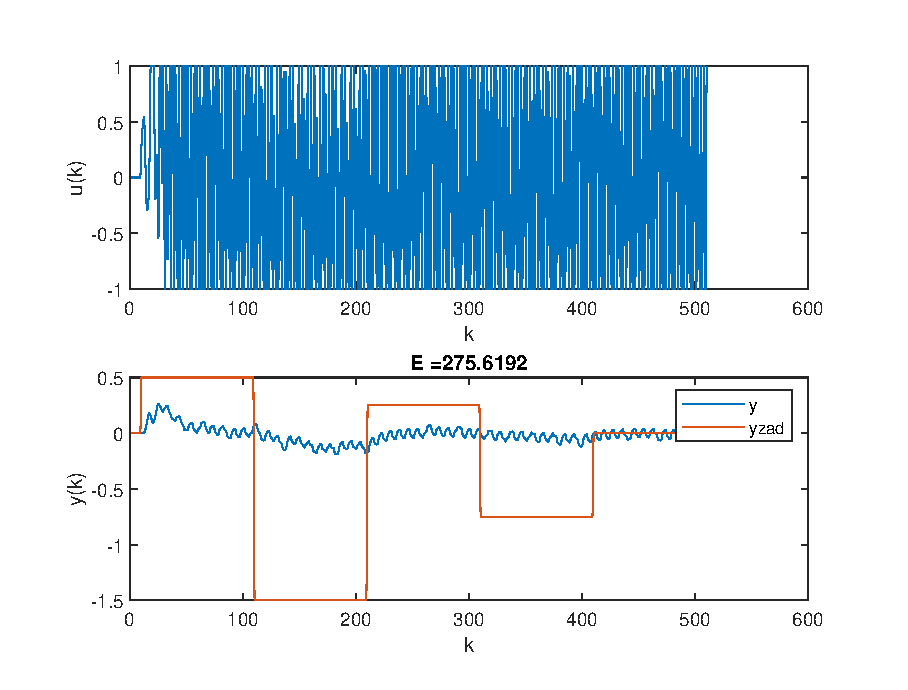
\includegraphics[width=\linewidth]{img/strojenieGPC_N_19_Nu_2_lam_4.eps}
			\caption{Działanie regulatora GPC z nastawami N=19, Nu=2, $\lambda$=4}
			\label{fig:GPC}
		\end{figure}
	
		\newpage
		Należy wziąć pod uwagę, że przez silną nieliniowość obiektu, liniowy algorytm GPC może generować duże sterowania, które po nałożeniu ograniczeń wprowadzą obiekt w stałe oscylacje. Można temu zapobiec poprzez zwiększenie współczynnika $\lambda$ o parę rzędów wielkości. Na rys. \ref{fig:GPC100} można zobaczyć, że jakość regulacji polepszyła się, lecz mimo to sterowanie wciąż jest zbyt ostre, a czas regulacji wolniejszy niż w przypadku NPL. W dodatku zarówno dla sterowania jak i wyjścia występują widoczne oscylacje.
		
		\begin{figure}[h!]
			\centering
			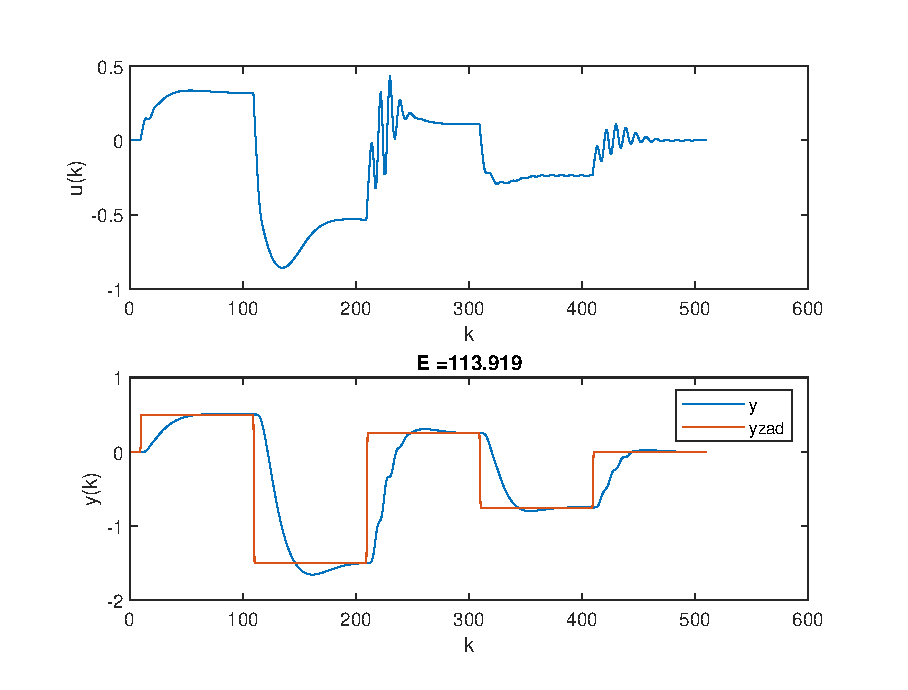
\includegraphics[width=\linewidth]{img/strojenieGPC_N_19_Nu_2_lam_100.eps}
			\caption{Działanie regulatora GPC z nastawami N=19, Nu=2, $\lambda$=100}
			\label{fig:GPC100}
		\end{figure}